\chapter{Stand der Technik}
\label{chap:Stand der Technik}

\section{Kinect}
% genaue Auflistung aller Bestandteile \ldots ben\"otigte Software, Eigenschaften
% Mikrofon, RGB-Kamera, Infrarot \ldots
Kinect ist ein Ger\"at zur Detektion von Bewegungen. Entwickelt wurde es von PrimeSense als Hardware zur Steuerung der Videokonsole 
XBOX 360 von Microsoft Corp. Nach der Ank\"undigung im M\"arz 2010 \footnote{Pressemitteilung, der Ver\"offentlichung. Siehe \href{https://www.microsoft.com/en-us/news/press/2010/mar10/03-31PrimeSensePR.aspx}{Link}. Microsoft.com.  Abgerufen Dezember 20, 2012}
war die Erweiterung mit dem Erscheinungsdatum 10. November 2010 in der Ausf\"uhrung \textit{Kinect for XBOX 360} in Europa erh\"altlich \footnote{Erscheinungsdatum der \textit{Kinect for XBOX 360}. Siehe \href{http://www.bbc.co.uk/newsbeat/10996389}{Link}. BBC UK. Abgerufen Dezember 20, 2012}.
Nach einem sehr erfolgreichem Verkaufsstart \footnote{\href{http://www.guinnessworldrecords.com/records-9000/fastest-selling-gaming-peripheral/}{\enquote{Am schnellsten verkauftes Perepherieger\"at f\"ur Spiele}}. Guinnessworldrecords.com. Abgerufen Dezemeber 22, 2012}
und anhaltender Nachfrage\footnote{Takahashi, Dean (Januar 9, 2012). \href{http://venturebeat.com/2012/01/09/xbox-360-surpassed-66m-sold-and-kinect-has-sold-18m-units/}{\enquote{Xbox 360 surpasses 66M sold and Kinect passes 18M units}}. venturebeat. Abgerufen Dezember 20, 2012},
k\"undigte Microsoft am 9. Januar 2012 ein weiteres Modell der Kinect, die sogenannte \textit{Kinect for Windows} f\"ur den 1. Februar 2012 an \footnote{\href{https://blogs.msdn.com/b/kinectforwindows/archive/2012/01/09/kinect-for-windows-commercial-program-announced.aspx?Redirected=true}{\enquote{Ank\"undigung der \textit{Kinect for Windows}}}. blogs.msdn.com. Abgerufen Dezember 22, 2012}.
\newline
Dar\"uber hinaus ver\"offentlichte Microsoft bereits am 16. Juni 2011 eine erste Version ihrer \textit{Kinect for Windows SDK}\footnote{\href{https://www.microsoft.com/en-us/news/press/2011/jun11/06-16MSKinectSDKPR.aspx}{\enquote{Microsoft Releases Kinect for Windows SDK Beta for Academics and Enthusiasts}}. Microsoft.com. Abgerufen Dezember 21, 2012}.
Mit diesem \gls{SDK} ist es m\"oglich auf einer Windows 7 Plattform Anwendungen zu entwickeln, die eine Kinect als Eingabeger\"at verwenden.
\newline
Mit der Verf\"ugbarkeit einer Kinect-Variante, die f\"ur den Einsatz am PC ausgelegt ist und der frei zug\"anglichen \glslink{SDK}{SDK} wurde diese zum Forschungsgegenstand, was auch der ausschlaggebende Punkt f\"ur den Einsatz der Kinect in dieser Studienarbeit ist.
\subsection{Hardware}
% Beschreibung und Vorgaben der genutzten Technik

Die beiden Kinect-Modelle unterscheiden sich in einigen Details\footnote{\href{https://www.microsoft.com/en-us/kinectforwindows/news/faq.aspx}{\enquote{Informationsseite \"uber Unterschiede der Kinect Versionen}}. Microsoft.com. Abgerufen Dezember 22, 2012}.
Der bedeutendste Faktor ist das sogenannte \textit{Near Mode} Feature:
\begin{quote}
Near Mode enables the depth sensor to see objects as close as 40 centimeters and also communicates more information about depth values outside the range than was previously available. There is also improved synchronization between color and depth, mapping depth to color, and a full frame API. \footnotemark[7]
\end{quote}
Neben dem aktualisierten Tiefensensor unterscheiden sich die beiden Varianten auch in einer h\"oheren Aufl\"osung der RGB-Kamera, die f\"ur eine Gestenerkennung relevant sein kann.
Aus diesem Grund wird f\"ur diese Arbeit die \textit{Kinect for Windows} genutzt.
\subsubsection{Technische Daten}
Eine Kinect ent\"alt innerhalb des Geh\"auses, folgende Sensoren \footnote{\href{http://msdn.microsoft.com/en-us/library/jj131033.aspx}{\enquote{Kinect for Windows Sensor Components and Specifications}}. msdn.microsoft.com. Abgerufen Dezember 21, 2012}:

\begin{figure}[htb]
\centering
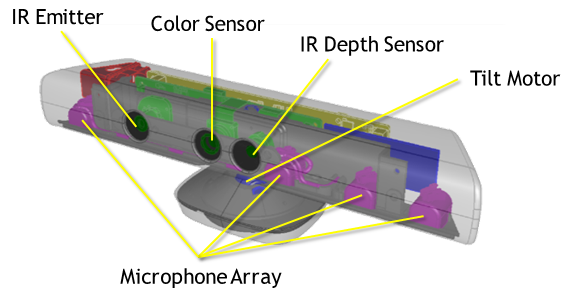
\includegraphics[width=0.8\textwidth]{img/kinect/kinect_interior.png}
\caption[Schematische Ansicht der Sensoren einer Kinect for Windows]{Schematische Ansicht der Sensoren einer \textit{Kinect for Windows} (Quelle: Microsoft Corp.\footnotemark[8])}
\label{fig:Schematische Ansicht der Sensoren einer Kinect for Windows}
\end{figure}

\begin{itemize}
  \item Eine RGB-Kamera mit einer Aufl\"osung von 1280x960.
  Dies erm\"oglicht eine Farbbilderfassung
  \item Ein Infrarot (IR) Emitter und ein IR Tiefensensor.
  Der Emitter emittiert infrarote Lichtstrahlen und der Tiefensensor erfasst die an den Sensor reflektierten Strahlen.
  Die reflektierten Strahlen werden in Tiefeninformation umgewandelt, in dem der Abstand zwischen Objekt und Sensor bestimmt wird.
  Dies erm\"oglicht die Erfassung von Tiefenbildern
  \item Ein \gls{Beamforming}, das vier Mikrofone zur Soundaufnahme enth\"alt. Die Anzahl der Mikrofone erm\"oglicht nicht nur die Aufzeichnung von Audiodaten,
  sondern auch die Lokalisierung der Soundquelle und die Richtung des Audiosignals
  \item Ein 3-Achsen-Beschleunigungssensor, konfiguriert f\"ur einen Bereich der zweifachen Erdbeschleunigung, um die gegenw\"artige Ausrichtung der Kinect zu bestimmen
  \item Ein Kippmotor, zur automatisierten Justierung der Sensoren
\end{itemize}

Weitere Details der technischen Spezifikation einer \textit{Kinect for Windows} sind in Tabelle~\ref{tab:Kinect - technische Spezifikation} aufgelistet:

\begin{table} [H] % \scriptsize
\begin{center}
\caption[Technische Spezifikation der Kinect for Windows]{Kinect for Windows -- technische Spezifikation \footnotemark[8]}
\label{tab:Kinect - technische Spezifikation}
\begin{tabular}{|p{5.7cm}|p{9cm}|}
\hline
\textbf{Kinect} & \textbf{Spezifikation} \\
\hline
Blickwinkel & $43\degree$ vertikales, $57\degree$ horizontales Blickfeld \\
\hline
Vertikaler Neigebereich & $\pm 27\degree$ \\
\hline
Bildwiederholrate (Farb- und Tiefensignal) & 30 Bilder pro Sekunde (FPS) \\
\hline
Audioformat & 16-kHz, 24-bit mono pulse code modulation (PCM)\\
\hline
Audioeingang & Ein Vier-\gls{Beamforming} mit 24-Bit Analog-Digital-Wandler (ADC)\\
\hline
Datensignal--Tiefensensor & 640x480 16-bit, 30 Bilder pro Sekunde \\
\hline
\multirow{2}{*}{Datensignal--RGB-Kamera} & 1280x960 16-Bit, 12 Bilder pro Sekunde\\
& 640x480 16-Bit, 30 Bilder pro Sekunde \\
\hline
Tiefensensorreichweite & 0,4 -- 4 m\\
\hline
\multirow{2}{*}{
\textit{\gls{Skeletal Tracking System}}} & Erkennung von bis zu sechs Benutzern, zwei davon trackbar/verfolgbar\\
& Verfolgung von 20 Gelenken pro aktivem Nutzer\\
\hline
\end{tabular}
\end{center}
\end{table}

\footnotetext[8]{\href{http://msdn.microsoft.com/en-us/library/jj131033.aspx}{\enquote{Kinect for Windows Sensor Components and Specifications}}. msdn.microsoft.com. Abgerufen Dezember 21, 2012}

\subsection{Software}
Durch die Ver\"offentlichung eines \glslink{SDK}{Software Development Kits} ist es m\"oglich, die Kinect in eigene Programme einzubinden und neue Anwendungsf\"alle zu bearbeiten.
Dazu hat Microsoft ebenfalls ein Handbuch ver\"offentlicht \cite{bib:kinect_hig}, das Informationen und Ratschl\"age zum Entwurf von Anwendungen liefert.
\subsubsection{Kinect for Windows SDK}
\label{subsubsec:Kinect_SDK}
% N\"otig f\"ur Steuerung der Kinect
Das \textit{Kinect for Windows SDK} steht aktuell in der Version 1.6 \footnote{\href{https://www.microsoft.com/en-us/kinectforwindows/develop/}{Downloadseite des SDK}. Microsoft.com. Abgerufen Dezember 21, 2012}
bereit. Dabei kann direkt in den Programmiersprachen C++, C\# , und Visual Basic auf einer Windows 7 Plattform entwickelt werden.
\newline
Das SDK umfasst dabei folgende Funktionen \footnote{\href{http://msdn.microsoft.com/en-us/library/hh855348.aspx}{\enquote{Kinect for Windows Programming Guide}}. msdn.microsoft.com. Abgerufen Dezember 23, 2012}:
\begin{itemize}
  \item Treiber und technische Dokumentation zur Implementierung von Anwendungen, die Kinect for Windows Sensoren nutzen
  \item Referenz APIs und Dokumentation zur Programmierung von \textit{managed} und \textit{unmanaged} Code.
  Die APIs stellen mehrere Mediensignale bereit
  \item Beispiele und Best-Practice-L\"osungen
\end{itemize}
\subsubsection{Weitere Frameworks}
Da Microsoft die Nutzungsm\"oglichkeiten seines SDK hinsichtlich verwendeter Programmiersprache und Plattform einschr\"ankt, begannen Forscher eigene Frameworks und Treiber zur Nutzung der Kinect zu entwickeln\footnote{\href{http://hackaday.com/2010/11/11/open-source-kinect-contest-has-been-won/}{\enquote{Open Source Kinect contest has been won}}. hackaday.com. November 11, 2010. Abgerufen Dezember 21, 2012}.
PrimeSense selbst ver\"offentlichte Treiber und Middleware f\"ur die Kinect \footnote{Mitchell, Richard (Dezember 10, 2010). \href{http://www.joystiq.com/2010/12/10/primesense-releases-open-source-drivers-middleware-for-kinect/}{\enquote{PrimeSense releases open source drivers, middleware for Kinect}}. Joystiq. Abgerufen Dezember 22, 2012}, 
als das offizielle SDK noch nicht zur Verf\"ugung stand.
\newline
Das Ziel dieser Frameworks war es zu meist, Kinect-Steuerung unter Unix-Plattformen und Programmiersprachen, wie Java, nutzbar zu machen.
Ein Teil dieser Ausarbeitung ist es, ein f\"ur die Aufgabenstellung und Zielsetzung der Studienarbeit passendes Framework zu bestimmen.
\newline
Verbreitete L\"osungen, die im Kapitel~\ref{chap:Kinect} n\"aher betrachtet werden, sind:
\begin{itemize}
  \item OpenNI
  \item OpenKinect
  \item jnect
\end{itemize}

\section{Java -- Eclipse}
% Entwicklungsumgebung \ldots
Die Anwendung, die im Rahmen dieser Arbeit entsteht, wird auf Basis der Programmiersprache Java und der Entwicklungsumgebung Eclipse erstellt.
Die Nutzung der Kinect und des Kinect SDK unterst\"utzt nativ nicht die Entwicklung auf Basis von Java, wie in Abschnitt~\ref{subsubsec:Kinect_SDK}
festgestellt wurde. Da jedoch die Expertise der Autoren dieser Arbeit im Java-Umfeld liegt, wird die Anwendung dennoch in der Programmiersprache Java umgesetzt.
\newline
Als Entwicklungsumgebung kommt die \gls{Eclipse} \acrshort{IDE} zum Einsatz. Diese bietet alle Voraussetzungen zur Entwicklung von flexiblen Java-Anwendungen und eine
ausf\"uhrliche Support-Plattform f\"ur Entwickler. Zus\"atzlich setzt es auf eine dynamische Supportplattform zur Modularisierung von Anwendungen\footnote{\href{http://eclipse.org/osgi/}{\enquote{OSGi}}. eclipse.org. Abgerufen Januar 1, 2013}.

\subsection{OSGi}
\label{subsec:OSGi}
Zur Entwicklung einer komplexen Anwendung mit vielen Abh\"angigkeiten und Schnittstellen, wie die hier zu erarbeitende, braucht es eine entsprechend \textit{m\"achtige} Software-Architektur. Dabei wird hier auf die OSGi-Plattform gesetzt.
OSGi\footnote{\href{http://www.osgi.org/Technology/HomePage}{\enquote{OSGi Alliance}}. osgi.org. Abgerufen Januar 1, 2013} ist ein \gls{Framework}, das Spezifikationen zur Definition eines dynamischen \textit{Komponentenmodells} unter Java bereitstellt.
Diese Komponenten werden \textit{Bundles} genannt und stehen anderen Komponenten als sogenannte \textit{Services} bereit.
Die OSGi Alliance\footnotemark[1] selbst spezifiziert lediglich die \gls{API}. Die Umsetzung f\"ur die Eclipse \acrshort{IDE} lautet \gls{Equinox}\footnote{\href{http://eclipse.org/equinox/}{\enquote{equinox OSGi}}. eclipse.org. Abgerufen Januar 1, 2013}.

\subsection{Grafische Oberfl\"ache}
% Darstellung der Anwendung, der Gesteneingabe etc.
Das \gls{GUI} ist ein wesentlicher Bestandteil der Anwendung, da hier\"uber der gesamte Informationsaustausch mit dem Nutzer der Kinect stattfindet.
Dabei wird auf verschiedene Techniken gesetzt, die im folgenden kurz beschrieben werden.
\newline
Bei der grafischen Darstellung muss man zwischen Informationen der Anwendung und Interaktion des Nutzers mit der Software unterscheiden. Dazu werden n\"amlich unterschiedliche Techniken verwendet.

\subsubsection{Rich client platform}
Die \gls{RCP} ist ein Werkzeug zur Entwicklung von unabh\"angigen Software-Komponenten, die nicht nur auf \acrshort{GUI}-Komponenten beschr\"ankt ist
\footnote{\href{http://wiki.eclipse.org/index.php/Rich_Client_Platform}{\enquote{Rich Client Platform}}. wiki.eclipse.org. Abgerufen Januar 1, 2013}.
Dabei liegt der Fokus auf einer Client-Applikation, worunter auch die Anwendung dieser Arbeit f\"allt.
Daher wird \acrshort{RCP} im Rahmen dieser Arbeit zur Erstellung der Oberf\"ache der Anwendung verwendet.
\subsubsection{Die Lightweight Java Game Library}
Die grafische Darstellung der Interaktion zwischen Akteur und Kinect ist ein wichtiger Bestandteil dieser Anwendung.
Zur Anzeige aufw\"andiger grafischer Objekte wird auf die \gls{LWJGL}\footnote{\href{http://www.lwjgl.org/}{\enquote{LWJGL Lightweight Java Game Library}}. lwjgl.org. Abgerufen Januar 1, 2013} gesetzt.
Damit k\"onnen einfach zweidimensionale Grafiken, zum Beispiel Kreise, oder komplexe dreidimensionale Ansichten in einer Java-Anwendung angezeigt werden.
Diese Java-Bibliothek stellt eine API zum Zugriff und zur Verwendung der bekannten \gls{OpenGL}\footnote{\href{https://www.opengl.org/}{\enquote{The Industry's Foundation for High Performance Graphics}}. opengl.org. Abgerufen Januar 1, 2013} bereit.

\subsubsection{Eclipse Modeling Framework}
Das \gls{EMF}\footnote{\href{http://www.eclipse.org/modeling/emf/}{\enquote{Eclipse Modeling Framework Project (EMF)}}. eclipse.org. Abgerufen Januar 1, 2013} ist ein Framework zur Modellierung von Java-Anwendungen.
Es erm\"oglicht aus strukturierten Datenmodellen, Java-Code zu generieren. F\"ur die Kinect-Anwendung sind lediglich die Bereiche des Frameworks relevant, die diese \textit{Modelle} beschreiben.
 
\subsubsection{Graphical Editing Framework}
Zur grafischen Darstellung und grafischen Manipulation der zuvor vorgestellten EMF-Modelle existiert das sogenannte \gls{GEF}\footnote{\href{http://www.eclipse.org/gef/}{\enquote{GEF (Graphical Editing Framework)}}. eclipse.org. Abgerufen Januar 1, 2013}.
Es stellt Methoden zur Verf\"ugung, um Grafikeditoren und weitere Ansichten f\"ur Eclipse Anwendungen zu erstellen. F\"ur die Studienarbeit relevante Bereiche, sind die Funktionen, die eine vereinfachte Darstellung der eben genannten EMF-Modelle erm\"oglichen.

\section {Roboter -- Ausblick}
% offene Schnittstelle, Arbeiten f\"ur 2. Studienarbeit \ldots
Ziel und Aufgabenstellung dieser Arbeit ist, wie bereits in Kapitel~\ref{chap:Aufgabenstellung} erl\"autert, der Entwurf einer Steuerung f\"ur einen mobilen Roboter.
Der erste Teil, der zweigeteilten Studienarbeit befasst sich dabei nicht direkt mit der eigentlichen Robotersteuerung oder der Beschreibung und Auswahl eines entsprechenden Modells.
Dies ist Aufgabe und Fokus des zweiten Teils.
\newline
F\"ur die Zwecke der Arbeiten an diesem Teil und der dabei zu erstellenden Anwendung, wird lediglich ein Grundger\"urst und eine Schnittstelle erarbeitet, um auf die Kinect-Steuerung zuzugreifen.
Siehe hierzu Abschnitt~\ref{subsec:Roboterschnittstelle}.
\section{Mustererkennung}
% kurzer Einblick in m\"ogliche Techniken/Techologien f\"ur Gestenerkennung \ldots
Die \textit{Kinect for Windows} und die dazu geh\"ohrende \textit{Kinect for Windows SDK} besitzen bereits Algorithmen zur Detektion von Bewegungen einzelner K\"orperteile und der Erkennung von Sprache.
Dabei muss festgehalten werden, dass zwischen der Detektion der Bewegung eines Gelenkes und der Erkennung einer Geste eine gro\ss e Diskrepanz besteht. Die Bewegung an sich macht noch keine Geste aus.
Zur \textit{Gestenerkennung} sind Verfahren und Algorithmen notwendig, die \"uber den Funktionsumfang der Kinect \acrshort{SDK} hinausgehen.
\newline
Hierzu sind Verfahren der Mustererkennung notwendig, die auf mathematischen Modellen beruhen. Dabei haben sich zwei Richtungen herausgebildet.
Eine Variante nutzt hierbei sogenannte \glspl{NeuroNetz}. Beschrieben und umgesetzt wurde dieser Ansatz unter anderem von Chun Zhu and Weihua Sheng~\cite{bib:neuralnetwork}.
\newline
Eine weitere Variante setzt das sogenannte \gls{HMM} ein, das von Leonard E. Baum~\cite{bib:hmmbaum} postuliert wurde. Dabei handelt es sich um ein stochastisches Modell, indem ein System durch eine Markov-Kette~(Siehe Abschnitt~\ref{subsec:MarkovKette}) modelliert wird. Eine der ersten Arbeiten zum Einsatz in der Gestenerkennung schrieb Lawrence R. Rabiner~\cite{bib:hmmrabiner}.
Dieser Ansatz findet h\"aufige Verwendung in Bereichen der Spracherkennung, Gestenerkennung und in der \glslink{MMS}{Mensch-Maschine-Kommunikation}. Aus diesem Grund wurde entschieden, ein \gls{HMM} zu erstellen.
Das stochastische Modell dahinter wird in Kapitel~\ref{chap:Modelle} und die Umsetzung in der Implementierung in Kapitel~\ref{chap:Implementierung} beschrieben.